\section{The System Behaviour Analysis}
\subsection{Purpose of Activity Diagrams}

Activity Diagrams are useful for depicting how each use case achieves its goal. They allow you to explicitly view the stakeholders involved, their roles and responsibilities and how they participate with activities within the context of the domain. Activity diagrams highlight the information stakeholders consume when they accomplish certain activities and aid in the identification of objects or information elements\cite{ibmactivity}. The basic purpose of an activity diagram is to show message flow from one activity to another. This details and includes the activity flow of the system, the sequence from one activity to another and the parallel or concurrent flow of the system\cite{lucidactivity}.

\begin{figure}[H]
    \centering
    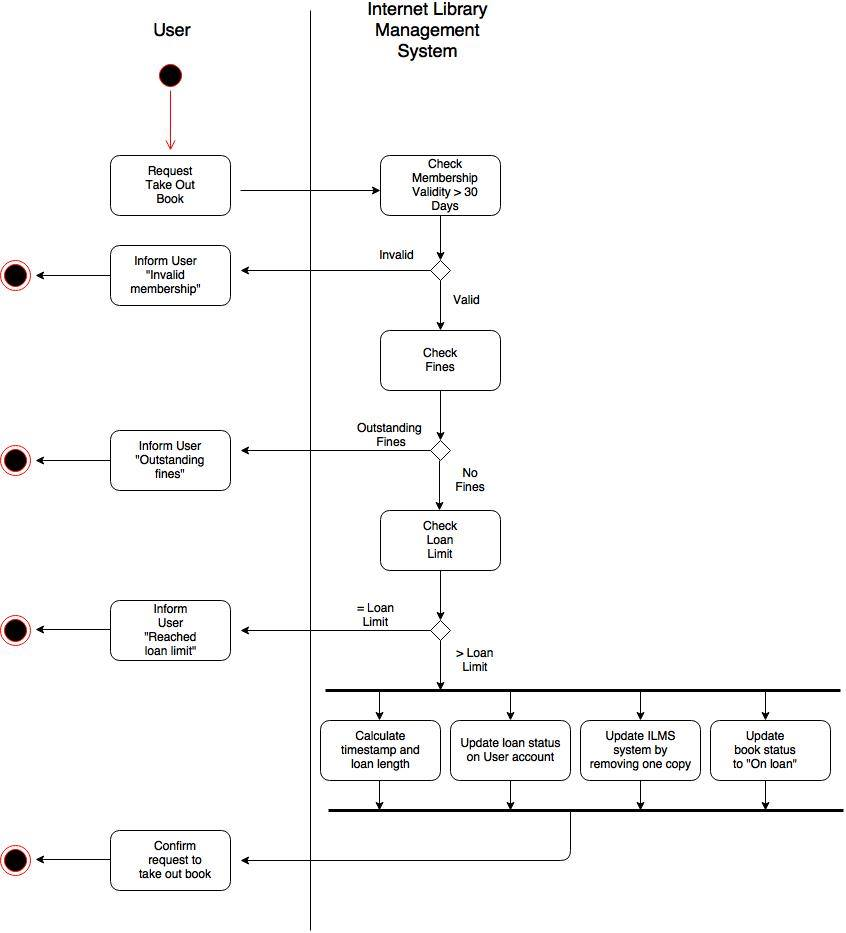
\includegraphics[width=0.75\linewidth]{image/activity.jpg}
    \caption{Activity Diagram}
    \label{fig:activity}
\end{figure}

The activity diagram for the ILMS shows actions for the use case of taking a book out. It includes steps that the user account must pass in order for the book to be taken out and has break cases where if a step fails, it will stop the book being taken out and will inform user of why the action cannot be performed. The user will simply need to make changes regarding a given error message to then be able to take out a book. 

When a user requests to take out a book, membership must be confirmed to be over 30 days, there must be no outstanding fines and the loan limit must not have been reached. Then multiple steps to update both the ILMS system and the user’s account will be carried out in parallel. Initially, a timestamp will be created which calculates when the user is due to return the book to the library. This timestamp is then allocated to the individual user’s account, and the user’s account is also updated to show the details of the book. When the loan status on the user’s account is updated, this will in turn increase the value of the asset relating to loan limit on the user’s account by 1. Furthermore the ILMS system will also be updated to detail that one copy of the book has been removed from the library. The individual copy of the book will also be updated in order to show that the book has now been placed on loan and is no longer available in the library. Once these steps have been carried out in parallel, the user will confirm the request to take out the book and all of the changes will be committed to the database.

The activity diagram has been designed to check these specific use cases as they were initially highlighted in the business rules. For example, if a user does not have a membership valid for more than 30 days, it is possible that they can return a book outside of their membership period, which should not be allowed. A user should also not be able to take out a book if they have any outstanding fines on their account, as then they could potentially just accrue more fines and never settle their account. Furthermore each user has a given loan limit, staff members can borrow 17 books, a postgraduate student 10 and undergraduate student 6. The limit for a member of the public is 6 books. Therefore loan limits must be checked against individual users in order to ensure that their limit has not been reached. As long as all of these conditions pass, a user will be able to confirm a request to take out a book. 

This model is used to aid the creation to the functional workflow design utilised in section 2.4 of this report. The output of this diagram is also useful for modelling the business requirements and allowing for a high level understanding of the system's functionality\cite{sourcemakingactivity}. This diagram has more impact upon business understanding than implementation details, however this is still partially used for implementation of the sequence model diagram. 